\documentclass[11pt,a4paper]{article}
\usepackage[T1]{fontenc}
\usepackage[utf8]{inputenc}
\usepackage{lmodern}
\usepackage{textcomp}
\usepackage[left=1.8cm,right=1.8cm,top=2.3cm,bottom=2.2cm,headheight=14pt,headsep=8pt]{geometry}
\usepackage{multicol}
\usepackage{xcolor}
\usepackage{fancyhdr}
\usepackage{graphicx}
\usepackage{array}
\usepackage{amsmath,amssymb}
\usepackage{setspace}
\usepackage{longtable}
\graphicspath{{../}}
\definecolor{ygreen}{RGB}{46,139,87}
\renewcommand{\normalsize}{\fontsize{10.9}{13.4}\selectfont}
\renewcommand{\familydefault}{\rmdefault}
\setlength{\parindent}{0pt}
\setlength{\columnsep}{0.8cm}
\setlength{\columnseprule}{0.4pt}
\setlength{\multicolsep}{3pt plus 1pt minus 1pt}
\renewcommand{\textsubscript}[1]{\ensuremath{_{\text{\fontsize{8}{8}\selectfont #1}}}}
\renewcommand{\textsuperscript}[1]{\ensuremath{^{\text{\fontsize{8}{8}\selectfont #1}}}}
\newcommand{\diqqat}[1]{\par\smallskip\noindent\textbf{Diqqat!} #1\par\medskip}
\newcommand{\javob}{\par\smallskip\noindent\textbf{Javob:} \rule[-2pt]{7.5cm}{0.4pt}\par\smallskip\noindent\textbf{Diqqat!} Javobingizni javoblar varaqasiga ko`chirib yozing.\par\medskip}
\pagestyle{fancy}
\fancyhf{}
\renewcommand{\headrulewidth}{0.4pt}
\fancyhead[L]{\textit{Milliy sertifikat 2026. Kimyo}}
\fancyhead[R]{17-variant}
\fancyfoot[L]{\fontsize{8}{9}\selectfont \textcopyright{} Colba maktabi, 2026}
\fancyfoot[C]{\thepage}
\fancypagestyle{first}{\fancyhf{}\renewcommand{\headrulewidth}{0pt}\fancyfoot[L]{\fontsize{8}{9}\selectfont \textcopyright{} Colba maktabi, 2026}\fancyfoot[C]{\thepage}}
\begin{document}
\normalsize
\thispagestyle{first}
\noindent\fcolorbox{ygreen}{white}{\parbox{\dimexpr\linewidth-2\fboxsep-2\fboxrule\relax}{%
\textbf{\fontsize{13}{15}\selectfont Nazorat testi}\ \textit{\fontsize{10}{12}\selectfont $\cdot$ Aralash test $\cdot$ 17-variant}\hfill
\begin{tabular}[t]{@{}r@{}}\textit{Milliy sertifikat 2026. Kimyo}\\ \textbf{\textit{\fontsize{8}{9}\selectfont Vaqt:}} \textit{\fontsize{10}{12}\selectfont 180 daqiqa}\end{tabular}}}
\par\medskip
\noindent\textit{Davriy jadvaldan foydalanish mumkin.}
\par\medskip
\begin{multicols}{2}
\noindent\textbf{1.} 3 mol Na\textsubscript{2}SO\textsubscript{4} va 2 mol K\textsubscript{3}PO\textsubscript{4} suvda eritilib, eritma hajmi 5 l ga yetkazildi. Eritmadagi barcha ionlarning umumiy molyar \textbf{konsentratsiyasini (mol/l) aniqlang} (kuchli elektrolitlar to`liq dissotsilanadi).

\noindent A)~\textsl{1} \hfill B)~\textsl{6,8} \hfill C)~\textsl{1,7} \hfill D)~\textsl{3,4}\par
\vspace{4pt}
\noindent\textbf{2.} 13,12 l He 127 \textdegree{}C va 1 atm bosimda necha gramm keladi? (R = 0,082 l$\cdot$atm/(mol$\cdot$K))

\noindent A)~\textsl{1,6} \hfill B)~\textsl{3,2} \hfill C)~\textsl{0,8} \hfill D)~\textsl{2,34}\par
\vspace{4pt}
\noindent\textbf{3.} 1 M Ca(OH)\textsubscript{2} eritmasining normal \textbf{konsentratsiyasini (n) aniqlang.}

\noindent A)~\textsl{1} \hfill B)~\textsl{4} \hfill C)~\textsl{2} \hfill D)~\textsl{0,5}\par
\vspace{4pt}
\noindent\textbf{4.} Quyidagi tuzlarning qaysilari suvli eritmasi kislotali muhitga ega? 1) CuSO\textsubscript{4}; 2) CH\textsubscript{3}COONa; 3) K\textsubscript{2}SO\textsubscript{4}; 4) Al\textsubscript{2}(SO\textsubscript{4})\textsubscript{3}

\noindent A)~\textsl{1, 4} \hfill B)~\textsl{3} \hfill C)~\textsl{2, 3, 4} \hfill D)~\textsl{1, 2, 4}\par
\vspace{4pt}
\noindent\textbf{5.} Jadvalda bog`lar hosil qiluvchi atomlarning elektrmanfiyliklari berilgan:
\begin{center}
\renewcommand{\arraystretch}{1.15}
\begin{tabular}{|c|c|c|}\hline
\textbf{Bog`} & \textbf{EM (1-atom)} & \textbf{EM (2-atom)} \\ \hline
C--H & 2,5 & 2,1 \\ \hline
H--O & 2,1 & 3,5 \\ \hline
Si--O & 1,8 & 3,5 \\ \hline
H--N & 2,1 & 3 \\ \hline
\end{tabular}
\end{center}
Qaysi bog` eng qutbli (eng ko`p ionli xarakterga ega)?

\noindent A)~\textsl{C--H} \hfill B)~\textsl{Si--O} \hfill C)~\textsl{H--O} \hfill D)~\textsl{H--N}\par
\vspace{4pt}
\noindent\textbf{6.} 56 g KOH 250 g suvda eritildi. Eritmaning molyal \textbf{konsentratsiyasini (mol/kg) aniqlang.}

\noindent A)~\textsl{3,27} \hfill B)~\textsl{0} \hfill C)~\textsl{8} \hfill D)~\textsl{4}\par
\vspace{4pt}
\noindent\textbf{7.} Faqat qaytaruvchi bo`la oladigan \textbf{ionlarni aniqlang}: 1) S\textsuperscript{2$-$}; 2) Al\textsuperscript{3+}; 3) Fe\textsuperscript{3+}; 4) Fe\textsuperscript{2+}

\noindent A)~\textsl{2, 4} \hfill B)~\textsl{1, 3} \hfill C)~\textsl{1} \hfill D)~\textsl{1, 2}\par
\vspace{4pt}
\noindent\textbf{8.} 14,3 g Na\textsubscript{2}CO\textsubscript{3}$\cdot$10H\textsubscript{2}O 200 g suvda eritildi. Eritmadagi tuzning massa \textbf{ulushini (\%) aniqlang.}

\noindent A)~\textsl{2,65} \hfill B)~\textsl{6,67} \hfill C)~\textsl{4,95} \hfill D)~\textsl{2,47}\par
\vspace{4pt}
\noindent\textbf{9.} Jadvalda CuSO\textsubscript{4} ning ikki eritmasi haqida ma'lumot berilgan:
\begin{center}
\renewcommand{\arraystretch}{1.15}
\begin{tabular}{|c|c|c|}\hline
\textbf{Eritma} & \textbf{Massasi, g} & \textbf{Massa ulushi, \%} \\ \hline
1 & 150 & 15 \\ \hline
2 & 300 & 25 \\ \hline
\end{tabular}
\end{center}
Eritmalar aralashtirilib, ustiga 50 g suv qo`shildi. Hosil bo`lgan eritmaning massa \textbf{ulushini (\%) aniqlang.}

\noindent A)~\textsl{20} \hfill B)~\textsl{40} \hfill C)~\textsl{19,5} \hfill D)~\textsl{18,33}\par
\vspace{4pt}
\noindent\textbf{10.} Elementning massa-spektri (izotoplar tarqalganligi) berilgan.
\begin{center}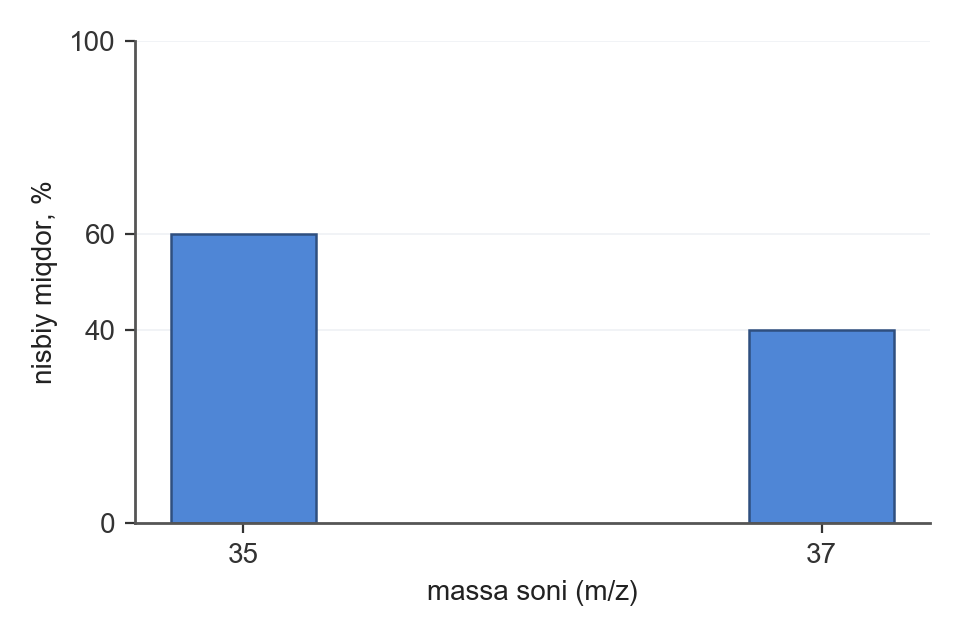
\includegraphics[width=0.86\linewidth]{rasmlar/gen/ms_v17_0.png}\end{center}
Elementning o`rtacha nisbiy atom \textbf{massasini aniqlang.}

\noindent A)~\textsl{64} \hfill B)~\textsl{64,6} \hfill C)~\textsl{63} \hfill D)~\textsl{63,4}\par
\vspace{4pt}
\noindent\textbf{11.} 2 g H\textsubscript{2} 127 \textdegree{}C va 1 atm bosimda qancha hajm (l) egallaydi? (R = 0,082 l$\cdot$atm/(mol$\cdot$K))

\noindent A)~\textsl{65,6} \hfill B)~\textsl{32,8} \hfill C)~\textsl{16,4} \hfill D)~\textsl{22,4}\par
\vspace{4pt}
\noindent\textbf{12.} Jadvalda S elementining birikmalaridagi oksidlanish darajasi berilgan:
\begin{center}
\renewcommand{\arraystretch}{1.15}
\begin{tabular}{|c|c|}\hline
\textbf{Modda} & \textbf{Oksidlanish darajasi} \\ \hline
H\textsubscript{2}S & -2 \\ \hline
Na\textsubscript{2}S & -2 \\ \hline
SO\textsubscript{3} & +6 \\ \hline
S & 0 \\ \hline
\end{tabular}
\end{center}
Ushbu moddalardan nechtasida S elementi faqat qaytaruvchi xossani namoyon qiladi? (S uchun eng past oksidlanish darajasi -2, eng yuqorisi +6)

\noindent A)~\textsl{3} \hfill B)~\textsl{4} \hfill C)~\textsl{2} \hfill D)~\textsl{5}\par
\vspace{4pt}
\noindent\textbf{13.} He va O\textsubscript{2} dan iborat 12,32 l (n.sh.) aralashmaning massasi 9,2 g. Aralashmadagi He ning \textbf{massasini (g) aniqlang.}

\noindent A)~\textsl{1} \hfill B)~\textsl{1,2} \hfill C)~\textsl{9,6} \hfill D)~\textsl{8}\par
\vspace{4pt}
\noindent\textbf{14.} KNO\textsubscript{3} tarkibidagi kaliy ning massa \textbf{ulushini (\%) aniqlang.}

\noindent A)~\textsl{38,6} \hfill B)~\textsl{19,3} \hfill C)~\textsl{77,2} \hfill D)~\textsl{2,6}\par
\vspace{4pt}
\noindent\textbf{15.} Reaksiya tenglamasi: 2NaNO\textsubscript{3} $\to$ 2NaNO\textsubscript{2} + O\textsubscript{2}. Reaksiyaga 170 g NaNO\textsubscript{3} kirishdi (unum 50\%). NaNO\textsubscript{2} \textbf{massasini (g) hisoblang.}

\noindent A)~\textsl{138} \hfill B)~\textsl{34,5} \hfill C)~\textsl{103,5} \hfill D)~\textsl{69}\par
\vspace{4pt}
\noindent\textbf{16.} SO\textsubscript{3} + H\textsubscript{2}O $\to$ H\textsubscript{2}SO\textsubscript{4} reaksiyasida 160 g SO\textsubscript{3} ishtirok etdi. H\textsubscript{2}SO\textsubscript{4} \textbf{miqdorini (mol) toping.}

\noindent A)~\textsl{4} \hfill B)~\textsl{1} \hfill C)~\textsl{2} \hfill D)~\textsl{3}\par
\vspace{4pt}
\noindent\textbf{17.} Reaksiya tenglamasi: N\textsubscript{2} + 3H\textsubscript{2} $\to$ 2NH\textsubscript{3}. Reaksiyaga 1 g H\textsubscript{2} kirishdi. NH\textsubscript{3} \textbf{hajmini (l, n.sh.) hisoblang.}

\noindent A)~\textsl{16,8} \hfill B)~\textsl{7,47} \hfill C)~\textsl{14,93} \hfill D)~\textsl{3,73}\par
\vspace{4pt}
\noindent\textbf{18.} 6,2 g fosfor yondirilib, hosil bo`lgan oksid suvda eritildi (ortofosfat kislota), so`ng 0,4 mol NaOH qo`shildi. Hosil bo`lgan Na\textsubscript{2}HPO\textsubscript{4} \textbf{massasini (g) aniqlang.}

\noindent A)~\textsl{56,8} \hfill B)~\textsl{28,4} \hfill C)~\textsl{14,2} \hfill D)~\textsl{24}\par
\vspace{4pt}
\noindent\textbf{19.} Cl\textsubscript{2} + 2NaOH $\to$ NaCl + NaClO + H\textsubscript{2}O reaksiyasida tarkibida 75\% aralashma bo`lgan 16 g namuna (asosiy modda NaOH) ishtirok etdi. NaCl \textbf{massasini (g) toping.}

\noindent A)~\textsl{2,93} \hfill B)~\textsl{11,7} \hfill C)~\textsl{5,85} \hfill D)~\textsl{1,46}\par
\vspace{4pt}
\noindent\textbf{20.} C\textsubscript{2}H\textsubscript{6} + Cl\textsubscript{2} $\to$ C\textsubscript{2}H\textsubscript{5}Cl + HCl jarayoni uchun 22,4 l (n.sh.) C\textsubscript{2}H\textsubscript{6} olingan (unum 75\%). HCl \textbf{hajmini (l, n.sh.) aniqlang.}

\noindent A)~\textsl{22,4} \hfill B)~\textsl{16,8} \hfill C)~\textsl{33,6} \hfill D)~\textsl{8,4}\par
\vspace{4pt}
\noindent\textbf{21.} CH\textsubscript{3}--CH(CH\textsubscript{3})--CH\textsubscript{2}--CH\textsubscript{3} birikmaning sistematik nomi qaysi qatorda to`g`ri keltirilgan?

\noindent\begin{tabular}{@{}p{0.47\linewidth}@{}p{0.47\linewidth}@{}}
A)~\textsl{2-metilbutan} & B)~\textsl{3-metilbutan} \\
C)~\textsl{2-etilpropan} & D)~\textsl{metilbutan} \\
\end{tabular}\par
\vspace{4pt}
\noindent\textbf{22.} Arenlar, neft va tabiiy gaz haqida qaysi fikrlar to`g`ri? 1) Naftalin -- bir halqali aren; 2) Benzoldan nitrobenzol nitrolash bilan olinadi; 3) Benzol uchun birikish reaksiyalari mutlaqo xos emas; 4) Benzol bromli suvni rangsizlantirmaydi

\noindent A)~\textsl{2, 4} \hfill B)~\textsl{1, 4} \hfill C)~\textsl{3} \hfill D)~\textsl{4}\par
\vspace{4pt}
\noindent\textbf{23.} CaC\textsubscript{2} + H\textsubscript{2}O reaksiyasi natijasida qaysi organik modda hosil bo`ladi?

\noindent\begin{tabular}{@{}p{0.47\linewidth}@{}p{0.47\linewidth}@{}}
A)~\textsl{etilen} & B)~\textsl{sirka kislota} \\
C)~\textsl{asetilen} & D)~\textsl{benzoy kislota} \\
\end{tabular}\par
\vspace{4pt}
\noindent\textbf{24.} 11 g CH\textsubscript{3}CHO dan quyidagi ikki bosqichda (CH\textsubscript{3}COO)\textsubscript{2}Ca olinadi: 1) CH\textsubscript{3}CHO + Ag\textsubscript{2}O $\to$ CH\textsubscript{3}COOH + 2Ag (unum 80\%); 2) 2CH\textsubscript{3}COOH + CaCO\textsubscript{3} $\to$ (CH\textsubscript{3}COO)\textsubscript{2}Ca + CO\textsubscript{2} + H\textsubscript{2}O (unum 80\%). Oxirgi mahsulot (CH\textsubscript{3}COO)\textsubscript{2}Ca ning \textbf{massasini (g) toping.}

\noindent A)~\textsl{12,64} \hfill B)~\textsl{15,8} \hfill C)~\textsl{19,75} \hfill D)~\textsl{25,28}\par
\vspace{4pt}
\noindent\textbf{25.} Rasmda organik birikmaning tuzilish formulasi keltirilgan.
\begin{center}
\includegraphics[width=0.86\linewidth]{rasmlar/gen/fg_987786.png}\end{center}
Molekuladagi uglerod atomlari \textbf{sonini aniqlang.}

\noindent A)~\textsl{4} \hfill B)~\textsl{2} \hfill C)~\textsl{3} \hfill D)~\textsl{5}\par
\vspace{4pt}
\noindent\textbf{26.} Murakkab efirlar va yog`lar haqida qaysi fikrlar to`g`ri? 1) Efirlanish reaksiyasi qaytmas; 2) Sovun --- yuqori yog` kislotalarning natriyli tuzi; 3) Etilatsetat efir hidli suyuqlik; 4) Murakkab efirlarning gidrolizi ishqoriy muhitda qaytmas

\noindent A)~\textsl{1, 2, 3} \hfill B)~\textsl{3, 4} \hfill C)~\textsl{2, 3, 4} \hfill D)~\textsl{2, 3}\par
\vspace{4pt}
\noindent\textbf{27.} Uglevodlar haqida qaysi fikrlar to`g`ri? 1) Kraxmal yod bilan ko`k rang beradi; 2) Saxaroza Feling suyuqligini qaytaradi; 3) Kraxmal va selluloza bir xil M ga ega; 4) Fruktoza ketospirt

\noindent A)~\textsl{2, 3} \hfill B)~\textsl{4} \hfill C)~\textsl{1, 2, 4} \hfill D)~\textsl{1, 4}\par
\vspace{4pt}
\noindent\textbf{28.} Aminlar, aminokislotalar va oqsillar haqida qaysi fikrlar to`g`ri? 1) Aminokislotalar amfoter birikmalar; 2) Oqsillar biuret reaksiyasini beradi; 3) Glitsin optik faol; 4) Aminokislotalar faqat kislotali xossaga ega

\noindent A)~\textsl{3, 4} \hfill B)~\textsl{1, 2} \hfill C)~\textsl{1, 2, 4} \hfill D)~\textsl{2, 4}\par
\vspace{4pt}
\noindent\textbf{29.} Vinilxlorid dan olingan polimerning polimerlanish darajasi 2500 bo`lsa, uning molyar \textbf{massasini (g/mol) aniqlang.}

\noindent A)~\textsl{78125} \hfill B)~\textsl{156250} \hfill C)~\textsl{312500} \hfill D)~\textsl{2562,5}\par
\vspace{4pt}
\noindent\textbf{30.} Kerosin va suv aralashmasi ni ajratish uchun qaysi usul mos?
\noindent A)~\textsl{suvda eritib, filtrlash, so`ng bug`latish}\par
\noindent B)~\textsl{bug`latish}\par
\noindent C)~\textsl{distillash (fraksiyalab haydash)}\par
\noindent D)~\textsl{ajratgich voronka}\par
\vspace{4pt}
\noindent\textbf{31.} Fenolftalein indikatori kislotali muhitda qanday rang beradi?

\noindent A)~\textsl{rangsiz} \hfill B)~\textsl{ko`k} \hfill C)~\textsl{binafsha} \hfill D)~\textsl{sariq}\par
\vspace{4pt}
\noindent\textbf{32.} Rasmda ammiakning suvda erishi ko`rsatilgan. 22,4 l (n.sh.) NH\textsubscript{3} 1000 g suvda eritilsa, eritmadagi ammiakning massa ulushi necha foiz?
\begin{center}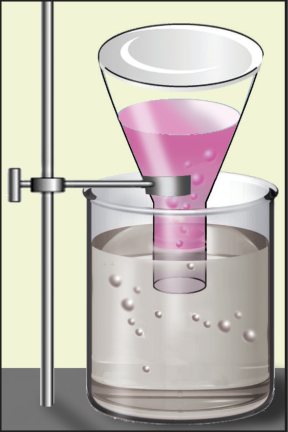
\includegraphics[width=0.86\linewidth]{rasmlar/darslik/d_nh3_fontan.png}\end{center}

\noindent\begin{tabular}{@{}p{0.47\linewidth}@{}p{0.47\linewidth}@{}}
A)~\textsl{1,7} & B)~\textsl{3,34} \\
C)~\textsl{0,84} & D)~\textsl{1,67   ---} \\
\end{tabular}\par
\vspace{4pt}
\end{multicols}
\medskip
\noindent\setlength{\fboxsep}{0pt}\fbox{\begin{tabular}{p{0.74\linewidth}|p{0.2\linewidth}}
\parbox[t]{0.72\linewidth}{\vspace{3pt}\textbf{Topshiriqlar (33--35) va javob variant (A--F)larini o`zaro to`g`ri moslashtiring.} Rux va magniy (Zn va Mg) dan iborat 24,3 g qotishma mo`l H\textsubscript{2}SO\textsubscript{4} eritmasida eritilganda 11,2 l (n.sh.) gaz ajraldi.
\vspace{3pt}} & \parbox[t]{0.19\linewidth}{\vspace{3pt}A~\textsl{72,3}\\[3pt]
B~\textsl{245}\\[3pt]
C~\textsl{490}\\[3pt]
D~\textsl{160,49}\\[3pt]
E~\textsl{367,5}\\[3pt]
F~\textsl{80,25}}\\ \hline
\parbox[t]{0.72\linewidth}{\vspace{2pt}\textbf{33. Qotishmadagi Zn massa ulushini (\%) aniqlang.}\vspace{2pt}} & \\ \hline
\parbox[t]{0.72\linewidth}{\vspace{2pt}\textbf{34. Reaksiya uchun sarflangan 20\% li H\textsubscript{2}SO\textsubscript{4} massasini (g) aniqlang.}\vspace{2pt}} & \\ \hline
\parbox[t]{0.72\linewidth}{\vspace{2pt}\textbf{35. Eritmadagi tuzlarning umumiy massasini (g) aniqlang.}\vspace{2pt}} & 
\end{tabular}}
\par\bigskip
\noindent\textbf{36.} Cu + HNO\textsubscript{3} $\to$ Cu(NO\textsubscript{3})\textsubscript{2} + NO\textsubscript{2} + H\textsubscript{2}O reaksiya tenglamasini tenglang va barcha koeffitsiyentlar \textbf{yig`indisini aniqlang.}
\javob
\noindent\textbf{37.} 24,5 g KClO\textsubscript{3} reaksiyaga kirishdi (2KClO\textsubscript{3} $\to$ 2KCl + 3O\textsubscript{2}). Ajralgan O\textsubscript{2} \textbf{hajmini (l, n.sh.) hisoblang} (unum 90\%).
\javob
\noindent\textbf{38.} NaBr va NaI dan iborat 17,8 g aralashma eritilib, mo`l xlor o`tkazildi, eritma bug`latilib quruq qoldiq 8,78 g chiqdi. Aralashmadagi NaI ning \textbf{massasini (g) toping.}
\javob
\noindent\textbf{39.} Etilatsetat va metilatsetat dan iborat 25 g aralashma mo`l NaOH eritmasi bilan to`liq gidrolizlandi. Hosil bo`lgan spirtlar umumiy \textbf{massasini (g) toping.}
\javob
\noindent\textbf{40.} 161,2 g tripalmitin gidrolizlanganda necha gramm glitserin hosil bo`ladi?
\javob
\par\bigskip\begin{center}\textbf{\fontsize{13}{15}\selectfont YOZMA ISH}\end{center}
\noindent\textbf{41.} \textbf{Topshiriqni bajarish jarayonida barcha reaksiya tenglamalarini yozing. Miqdoriy va arifmetik hisoblashlarni (unga asos bo`lgan usul yoki formulani ko`rsatgan holda) uzviy ketma-ketlikda bajaring.}\par\smallskip
Ketma-ket ulangan ikkita elektrolizyorda CuCl\textsubscript{2} va AgNO\textsubscript{3} eritmalari inert elektrodlar bilan elektroliz qilindi. Birinchi elektrolizyorning katodida 3,2 g Cu ajraldi (F = 96500 C/mol).\par
\noindent 1)Elektrolizyordan o`tgan zaryad miqdorini (C) hisoblang.\par
\noindent 2)Tok kuchi 10 A bo`lsa, elektroliz necha sekund davom etgan? O`tgan elektronlar miqdorini (mol) ham toping.\par
\noindent 3)Ikkinchi elektrolizyorning katodida ajralgan Ag massasini (g) aniqlang.\par
\noindent 4)Birinchi elektrolizyor anodida ajralgan gaz hajmini (l, n.sh.) toping. Ikkinchi elektrolizyor katodida ajralgan metallning miqdorini (mol) ham toping.\par
\noindent 5)Ikkala elektrolizyorda o`tgan elektronlar sonini (mol) taqqoslab, ularning teng ekanligini isbotlang. Agar tok kuchi 2 marta oshirilsa, shuncha zaryad o`tishi uchun necha sekund kerak?\par
\diqqat{Mazkur topshiriq kengaytirilgan javobni talab etib, uning yechilish usuli va shu usul asosidagi barcha hisoblash amallari javoblar varaqasida aks etishi lozim.}
\noindent\textbf{42.} Quyidagi o`zgarishlar zanjirida \textit{X}, \textit{Y}, \textit{Z} noma'lum organik moddalar:\par
\[\setlength{\fboxsep}{0pt}\text{CH\textsubscript{3}Cl}\xrightarrow{\text{Na}}\text{\textit{X}}\xrightarrow{\text{Cl\textsubscript{2}, yorug`lik}}\text{\textit{Y}}\xrightarrow{\text{KOH (spirtli)}}\text{\textit{Z}}\xrightarrow{\text{polimerlanish}}\text{(--CH\textsubscript{2}--CH\textsubscript{2}--)n}\]
\noindent 1)CH\textsubscript{3}Cl $\to$ \textit{X} : reaksiya tenglamasini yozing; hosil bo`lgan moddani nomlang.\par
\noindent 2)\textit{X} $\to$ \textit{Y} : reaksiya tenglamasini yozing; hosil bo`lgan moddani nomlang.\par
\noindent 3)\textit{Y} $\to$ \textit{Z} : reaksiya tenglamasini yozing; hosil bo`lgan moddani nomlang.\par
\noindent 4)\textit{Z} $\to$ (--CH\textsubscript{2}--CH\textsubscript{2}--)n : reaksiya tenglamasini yozing; hosil bo`lgan moddani nomlang.\par
\diqqat{Mazkur topshiriq kengaytirilgan javobni talab etib, uning yechilish usuli va shu usul asosidagi barcha hisoblash amallari javoblar varaqasida aks etishi lozim.}
\noindent\textbf{43.} \textbf{Topshiriqni bajarish jarayonida barcha reaksiya tenglamalarini yozing. Miqdoriy va arifmetik hisoblashlarni (unga asos bo`lgan usul yoki formulani ko`rsatgan holda) uzviy ketma-ketlikda bajaring.}\par\smallskip
SO\textsubscript{2} va CO\textsubscript{2} dan iborat 4,48 l (n.sh.) gazlar aralashmasi avval mo`l bromli suvdan, so`ngra mo`l Ba(OH)\textsubscript{2} eritmasidan o`tkazildi. Bromli suvdan o`tgandan keyin SO\textsubscript{2} to`liq yutildi.\par
\noindent 1)Bromli suv bilan SO\textsubscript{2} reaksiyasi tenglamasini yozing (SO\textsubscript{2} + Br\textsubscript{2} + 2H\textsubscript{2}O $\to$ H\textsubscript{2}SO\textsubscript{4} + 2HBr). Hosil bo`lgan H\textsubscript{2}SO\textsubscript{4} massasini (g) toping. SO\textsubscript{2} hajmini (l, n.sh.) ham hisoblang.\par
\noindent 2)Mo`l BaCl\textsubscript{2} qo`shilganda bromli suvli eritmada hosil bo`lgan cho`kma massasini (g) aniqlang.\par
\noindent 3)Ba(OH)\textsubscript{2} eritmasida hosil bo`lgan cho`kma massasini (g) hisoblang.\par
\noindent 4)Dastlabki aralashmaning o`rtacha molyar massasini (g/mol) va havoga nisbatan zichligini toping.\par
\noindent 5)Bromli suvli eritmada hosil bo`lgan HBr massasini (g) hisoblang.\par
\diqqat{Mazkur topshiriq kengaytirilgan javobni talab etib, uning yechilish usuli va shu usul asosidagi barcha hisoblash amallari javoblar varaqasida aks etishi lozim.}
\newpage
\noindent\textbf{\fontsize{13}{15}\selectfont Nazorat testi}\ \textit{$\cdot$ 17-variant}\hfill \textbf{Javoblar kaliti}\par\smallskip\hrule\smallskip
\textit{Faqat o`qituvchi uchun.}\par\medskip
\noindent\textbf{1--32-savollar}\par\smallskip
\noindent\begin{tabular}{|c|c|c|c|c|c|c|c|c|c|c|c|c|c|c|c|}\hline
\textbf{1} & \textbf{2} & \textbf{3} & \textbf{4} & \textbf{5} & \textbf{6} & \textbf{7} & \textbf{8} & \textbf{9} & \textbf{10} & \textbf{11} & \textbf{12} & \textbf{13} & \textbf{14} & \textbf{15} & \textbf{16}\\\hline
\textsl{D} & \textsl{A} & \textsl{C} & \textsl{A} & \textsl{B} & \textsl{D} & \textsl{C} & \textsl{D} & \textsl{C} & \textsl{D} & \textsl{B} & \textsl{C} & \textsl{B} & \textsl{A} & \textsl{D} & \textsl{C}\\\hline
\textbf{17} & \textbf{18} & \textbf{19} & \textbf{20} & \textbf{21} & \textbf{22} & \textbf{23} & \textbf{24} & \textbf{25} & \textbf{26} & \textbf{27} & \textbf{28} & \textbf{29} & \textbf{30} & \textbf{31} & \textbf{32}\\\hline
\textsl{B} & \textsl{B} & \textsl{A} & \textsl{B} & \textsl{A} & \textsl{A} & \textsl{C} & \textsl{A} & \textsl{C} & \textsl{C} & \textsl{D} & \textsl{B} & \textsl{B} & \textsl{D} & \textsl{A} & \textsl{D}\\\hline
\end{tabular}\par\medskip
\noindent\textbf{33--35-savollar}\par\smallskip
\noindent\begin{tabular}{|c|c|c|}\hline \textbf{No} & \textbf{Javob} & \textbf{Qiymat}\\\hline
33 & \textsl{F} & 80,25\\\hline
34 & \textsl{B} & 245\\\hline
35 & \textsl{A} & 72,3\\\hline
\end{tabular}\par\medskip
\noindent\textbf{36--40-savollar}\par\smallskip
\noindent\begin{tabular}{|c|c|}\hline \textbf{No} & \textbf{To`g`ri javob}\\\hline
36 & 10\\\hline
37 & 6,05\\\hline
38 & 7,5\\\hline
39 & 12,4\\\hline
40 & 18,4\\\hline
\end{tabular}\par\medskip
\noindent\textbf{41--43-topshiriqlar: qisqa yechim}\par\smallskip
\noindent\textbf{41-topshiriq.}\par
\noindent 1) n(Cu) = 0,05 mol; Q = n$\cdot$z$\cdot$F = 0,05$\cdot$2$\cdot$96500 = \textbf{9650 C}\par
\noindent 2) t = Q/I = 9650/10 = \textbf{965 s}; n(e\textsuperscript{$-$}) = Q/F = \textbf{0,1 mol}\par
\noindent 3) n(e\textsuperscript{$-$}) = 0,1 mol; n(Ag) = 0,1/1 = 0,1 mol $\to$ \textbf{10,8 g}\par
\noindent 4) Cl\textsubscript{2}: n = 0,05 mol $\to$ \textbf{1,12 l}; n(Ag) = \textbf{0,1 mol}\par
\noindent 5) Ketma-ket ulanishda har bir elektrolizyordan bir xil zaryad o`tadi: n(e\textsuperscript{$-$}) = 0,1 mol ikkala holda; t = 965/2 = \textbf{482 s}\par
\noindent Jami: M 15 + A 10 = 25 ball.\par
\noindent\textbf{42-topshiriq.}\par
\noindent 1) CH\textsubscript{3}Cl + Na $\to$ C\textsubscript{2}H\textsubscript{6} (etan)\par
\noindent 2) C\textsubscript{2}H\textsubscript{6} + Cl\textsubscript{2}, yorug`lik $\to$ C\textsubscript{2}H\textsubscript{5}Cl (xloretan)\par
\noindent 3) C\textsubscript{2}H\textsubscript{5}Cl + KOH (spirtli) $\to$ C\textsubscript{2}H\textsubscript{4} (etilen)\par
\noindent 4) C\textsubscript{2}H\textsubscript{4} + polimerlanish $\to$ (--CH\textsubscript{2}--CH\textsubscript{2}--)n (polietilen)\par
\noindent Jami 25 ball.\par
\noindent\textbf{43-topshiriq.}\par
\noindent 1) n(SO\textsubscript{2}) = 0,1 mol $\to$ n(H\textsubscript{2}SO\textsubscript{4}) = 0,1 mol $\to$ \textbf{9,8 g}; \textit{V}(SO\textsubscript{2}) = 0,1$\cdot$22,4 = \textbf{2,24 l}\par
\noindent 2) H\textsubscript{2}SO\textsubscript{4} + BaCl\textsubscript{2} $\to$ BaSO\textsubscript{4}$\downarrow$ + 2HCl: \textbf{23,3 g}\par
\noindent 3) CO\textsubscript{2} + Ba(OH)\textsubscript{2} $\to$ BaCO\textsubscript{3}$\downarrow$ + H\textsubscript{2}O: 0,1 mol$\cdot$197 = \textbf{19,7 g}\par
\noindent 4) M = (0,1$\cdot$64 + 0,1$\cdot$44)/0,2 = \textbf{54 g/mol}; D(havo) = 54/29 = \textbf{1,86}\par
\noindent 5) SO\textsubscript{2} + Br\textsubscript{2} + 2H\textsubscript{2}O $\to$ H\textsubscript{2}SO\textsubscript{4} + 2HBr: n(HBr) = 2$\cdot$0,1 = 0,2 mol $\to$ \textbf{16,2 g}\par
\noindent Jami: M 15 + A 10 = 25 ball.\par
\par\bigskip\noindent\textbf{Mavzular taqsimoti}\par\smallskip
{\small\noindent\begin{longtable}{|c|p{7.2cm}|p{5.4cm}|c|}\hline \textbf{No} & \textbf{Mavzu} & \textbf{Tekshiriladigan ko`nikma} & \textbf{Ball}\\\hline
1 & Tirkashev IV bob (kuchli elektrolitlar) & Hisoblash va masala yechish & 1\\\hline
2 & 11-sinf (Mendeleyev--Klapeyron) & Hisoblash va masala yechish & 1\\\hline
3 & 11-sinf 4-bob (normal konsentratsiya) & Hisoblash va masala yechish & 1\\\hline
4 & 9-sinf (gidroliz); Tirkashev IV bob & Bilim va tushunish & 1\\\hline
5 & 8-sinf (kimyoviy bog`lanish turlari, jadval) & Jadval tahlili & 1\\\hline
6 & 11-sinf 4-bob (molyal konsentratsiya) & Hisoblash va masala yechish & 1\\\hline
7 & Tirkashev \textit{V} bob; 11-sinf 7-bob & Bilim va tushunish & 1\\\hline
8 & Tirkashev III bob (kristallogidrat) & Hisoblash va masala yechish & 1\\\hline
9 & Tirkashev III bob (eritmalar, jadval) & Jadval tahlili & 1\\\hline
10 & 8-sinf (izotoplar, massa-spektr) & Grafik tahlili & 1\\\hline
11 & 11-sinf (Mendeleyev--Klapeyron) & Hisoblash va masala yechish & 1\\\hline
12 & Tirkashev \textit{V} bob (OQR, jadval) & Jadval tahlili & 1\\\hline
13 & 11-sinf (gaz aralashmalar) & Hisoblash va masala yechish & 1\\\hline
14 & Tashev (o`g`itlar) & Hisoblash va masala yechish & 1\\\hline
15 & 9-sinf; Tirkashev (tuzlarning termik parchalanishi, hisob) & Hisoblash va masala yechish & 1\\\hline
16 & 9-sinf; Tirkashev (S/SO\textsubscript{2}/H\textsubscript{2}SO\textsubscript{4}, hisob) & Hisoblash va masala yechish & 1\\\hline
17 & 9-sinf; Tirkashev (N/NH\textsubscript{3}/HNO\textsubscript{3}, hisob) & Hisoblash va masala yechish & 1\\\hline
18 & Tashev (fosfor) & Hisoblash va masala yechish & 1\\\hline
19 & 9-sinf; Tirkashev (galogenlar, hisob) & Hisoblash va masala yechish & 1\\\hline
20 & 10-sinf (alkan, hisob) & Hisoblash va masala yechish & 1\\\hline
21 & 10-sinf (nomenklatura \S{}6, \S{}11, \S{}20, \S{}24--26) & Bilim va tushunish & 1\\\hline
22 & 10-sinf (mavzuga oid paragraflar); Abdusamatov & Bilim va tushunish & 1\\\hline
23 & 10-sinf (olinish usullari) & Bilim va tushunish & 1\\\hline
24 & 10-sinf (ikki bosqichli hisob) & Hisoblash va masala yechish & 1\\\hline
25 & 10-sinf (organik birikmalar) & Rasm bo`yicha tahlil & 1\\\hline
26 & 10-sinf (mavzuga oid paragraflar); Abdusamatov & Bilim va tushunish & 1\\\hline
27 & 10-sinf (mavzuga oid paragraflar); Abdusamatov & Bilim va tushunish & 1\\\hline
28 & 10-sinf (mavzuga oid paragraflar); Abdusamatov & Bilim va tushunish & 1\\\hline
29 & 10-sinf \S{}35 (YuMB) & Hisoblash va masala yechish & 1\\\hline
30 & 7-sinf (aralashmalarni ajratish usullari) & Bilim va tushunish & 1\\\hline
31 & 8-sinf (indikatorlar) & Bilim va tushunish & 1\\\hline
32 & 8-sinf (24-rasm; eritmalar) & Rasm bo`yicha tahlil & 1\\\hline
33--35 & Aralash masala (moslashtirish) & Ko`p bosqichli hisob & 3\\\hline
36--40 & Qisqa javobli masalalar & Hisoblash & 5\\\hline
41--43 & Yozma ish & Usul va hisob (M, A) & 75\\\hline
\end{longtable}}
\end{document}
